\newcommand{\econtexRoot}{.}
% The \commands below are required to allow sharing of the same base code via Github between TeXLive on a local machine and ShareLaTeX.  This is an ugly solution to the requirement that custom LaTeX packages be accessible, and that ShareLaTeX seems to ignore symbolic links (even if they are relative links to valid locations)
\providecommand{\econtex}{\econtexRoot/texmf-local/tex/latex/econtex}
\providecommand{\econtexSetup}{\econtexRoot/texmf-local/tex/latex/econtexSetup}
\providecommand{\econtexShortcuts}{\econtexRoot/texmf-local/tex/latex/econtexShortcuts}
\providecommand{\econtexBibMake}{\econtexRoot/texmf-local/tex/latex/econtexBibMake}
\providecommand{\econtexBibStyle}{\econtexRoot/texmf-local/bibtex/bst/econtex}
\providecommand{\notes}{\econtexRoot/texmf-local/tex/latex/handout}
\providecommand{\handoutSetup}{\econtexRoot/texmf-local/tex/latex/handoutSetup}
\providecommand{\handoutShortcuts}{\econtexRoot/texmf-local/tex/latex/handoutShortcuts}
\providecommand{\handoutBibMake}{\econtexRoot/texmf-local/tex/latex/handoutBibMake}
\providecommand{\handoutBibStyle}{\econtexRoot/texmf-local/bibtex/bst/handout}

  
\documentclass[titlepage]{\econtex}\newcommand{\texname}{ConsumptionHeterogeneity}
\usepackage{\econtexSetup}\usepackage{\econtexShortcuts}
\usepackage[nolists,nomarkers,tablesonly]{endfloat}
\usepackage{tikz}
\usepackage{caption}
\usepackage{titlesec}
\setcounter{secnumdepth}{4}
\usepackage{placeins}
\usepackage{pdfpages}
\usepackage{setspace}
\usepackage{breqn}
\onehalfspacing

\usepackage{booktabs,rotating}

\titleformat{\paragraph}
{\sffamily\mdseries\normalsize}{\theparagraph}{1em}{}
\titlespacing*{\paragraph}
{0pt}{3.25ex plus 1ex minus .2ex}{1.5ex plus .2ex}



\begin{document}\bibliographystyle{\econtexBibStyle}
\input Switches.tex

\begin{verbatimwrite}{\jobname.title}
Sufficient Statistics in HANK
\end{verbatimwrite}

%\hfill{\tiny \jobname}

\title{ 
	\bigskip
	\bigskip
	Sufficient Statistics in HANK \\ A Paper Proposal}

\author{
  Edmund Crawley\authNum   \\ {\small JHU}
  \and
  Seungcheol Lee\authNum    \\ {\small UCL}
}


\keywords{}
\jelclass{}

\date{March 2019}
\maketitle


\begin{abstract}
\cite{auclert_monetary_2017} shows that, under certain conditions, the transmission of monetary policy can be decomposed into five partial equilibrium channels. This paper examines how useful this decomposition is in more general models, both TANK and HANK, which have more complex dynamics. We show that if the monetary policy shock is transitory, and with reasonably calibrated convex investment adjustment costs, the decomposition works well. Furthermore, we show that the current generation of TANK and HANK models do a poor job at matching the joint distribution of unhedged interest rate exposure and MPC. We suggest improving these models along this dimension is of primary quantitative importance.
\end{abstract}


\begin{authorsinfo}
\name{Crawley: Department of Economics, Johns Hopkins University, \href{mailto:ecrawle2@jhu.edu}{\texttt{ecrawle2@jhu.edu}}}
\name{Lee: University College London, \href{mailto:seungcheol.lee@ucl.ac.uk}{\texttt{seungcheol.lee@ucl.ac.uk}}}
\end{authorsinfo}

\titlepagefinish
\setcounter{page}{1}

\pagebreak
\section{Introduction}
A recent wave of so-called HANK models (Heterogeneous Agent New Keynesian) purport to show that the transmission mechanism of monetary policy may be very different to that of traditional New Keynesian models. While these models have generated much discussion, their quantitative relevance and importance for policy have yet to be proven. Indeed \cite{dgHANKTANK} claim that under certain conditions a simple TANK (Two Agent New Keynesian) model can suffice.

In a related paper, \cite{auclert_monetary_2017} shows how the transmission mechanism of monetary policy can be decomposed into five partial equilibrium channels, all of which are potentially measurable in data. The validity of the sufficient statistics he identifies rests on the assumption that an interest rate shock is transitory in nature.\footnote{Specifically, from the point of view of an individual household, a monetary policy shock consists of a transitory change in income, a permanent change in the price level and a transitory change to the real interest rate.}

This paper investigates how useful Auclert's sufficient statistics are in more general models where the exact conditions required for the decomposition do not hold. We will restrict ourselves to models where the interest rate depends only on the current economic conditions, so there is no `artificial' persistence in the interest rate. This is required to replicate the conditions for a transitory monetary policy shock.

We start with a basic TANK model in which the conditions for the sufficient statistics to exactly measure the transmission mechanism hold. We then extend the model in a variety of directions, including a simple HANK model.

Finally we show that the current generation of HANK models does not do a good job at matching the empirically measured joint distribution of unhedged interest rate exposure and MPCs.

\subsection{some notes...}
The key to the paper will be to show that there is no significant medium term dynamics in these models, once we disallow persistence in the shock itself ($\rho = 0$ for the interest rate shock). While this lack of persistence limits our study somewhat, we would also question how well these models capture consumption behavior with respect to future income/interest rates. There is a wealth of micro evidence to suggest that households respond to income \textit{when they get it}, not when they hear about it, which greatly brings into question the validity of the dynamics of these models. The advantage of limiting ourselves to models with little persistence is that we can stay close to what we know about the empirics.

The fact that households don't respond to income until they actually receive it seems likely to be the reason monetary policy seems to act with a delay (for example rates take time to adjust).

\section{Transmission Channels} \label{transmission_channels}

\section{A TANK Model in which the Sufficient Statistics Work Exactly}
Key features of model (I think):
\begin{itemize}
	\item Two agent, one unconstrained, one constrained
	\item Fixed amount of capital, K, all held by unconstrained agent
	\item Nominal bonds - either issued by government, or in net zero supply
	\item Borrowing constraint - either at zero, or cannot borrow more than some fraction of next period's income
	\item Government rebates any extra revenue via lump sum tax rebates.
	\item NK setup standard otherwise
\end{itemize}
I believe this model should fit Auclert's conditions exactly.\\
\\
\subsection{Model intro...}
Our baseline TANK model is composed of type types of agents, Ricardian and Keynesian, along with a continuum of intermediate goods firms, a perfectly competitive final goods firm, and a monetary policy authority. The model is closely related to the standard New Keynesian model with Calvo pricing frictions, the main difference being the addition of the Keynesian households. A key addition in our model is to allow for the Keynesian households to hold a non-zero quantity of short term nominal debt (owed to the Ricardian households) so that we have non-trivial levels for households' unhedged interest rate exposure (URE) and net nominal positions (NNP).

\subsection{Households}
A proportion $\lambda$ of households, which we shall call Keynesian, live hand-to-mouth, consuming all their income in each period. The remaining ($1-\lambda$), which we shall call Ricardian, are unconstrained optimizing agents.

\subsubsection{Ricardian Households}
Each period Ricardian households choose how much to consume, $C^R_t$, and how many hours to work, $N^R_t$ in order to maximize their life time (separable) utility:
\begin{align*}
\mathbb{E}\sum_{t=0}^{\infty}\beta^t \left(\frac{\left(C^R_t\right)^{1-\sigma}}{1-\sigma} - \frac{\left(N^R_t\right)^{1+\psi}}{1+\psi}\right)
\end{align*}
subject to their budget constraint:
\begin{align*}
P_t C^R_t + I_{t}^{-1}B_{t+1} =  N^R_t W_t + P_t D_t + B_t
\end{align*}
where $P_t$ is the price level in period $t$, $I_t$ is the gross nominal interest rate between $t$ and $t+1$, $B_t$ is the quantity of bonds bought at time $t-1$ paying one unit of nominal currency in period $t$, $W_t$ is the nominal wage per unit of labor in period $t$ and $D_t$ is the real dividend payed by firms in period $t$. All firm profit goes to the Ricardian households and this is shared equally between them.

The first order conditions for these Ricardian households are:
\begin{align}
\frac{W_t}{P_t} = \left(C^R_t\right)^{\sigma}\left(N^R_t\right)^{\psi} \label{foc_hours_R} \\
\left(C^R_t\right)^{-\sigma} = \beta \mathbb{E}\left(I_t\frac{P_{t}}{P_{t+1}} \left(C^R_{t+1}\right)^{-\sigma}\right)	\label{euler_R}
\end{align}

\subsubsection{Keynesian Households}
Keynesian households are more impatient that the Ricardian households and as a result are up against their borrowing limit. They can borrow nominal bonds up to the point where their expected \textit{real} payment in the next period is equal to a fixed fraction $\Omega$ of their steady state income. Each period they optimize their period utility:
\begin{align*}
\frac{\left(C^K_t\right)^{1-\sigma}}{1-\sigma} - \frac{\left(N^K_t\right)^{1+\psi}}{1+\psi}\
\end{align*}
subject to their budget constraint:
\begin{align}
C^K_t \leq N^K_t \frac{W_t}{P_t} + \left(I_{t}^{-1} \frac{\mathbb{E}_t P_{t+1}}{P_t} -  \frac{\mathbb{E}_{t-1}P_t }{P_t}\right)\Omega \bar{N_K}\overline{W/P}  \label{budget_constraint_K}
\end{align}
where $\overline{W/P}$ and $\bar{N_K}$ are the steady state real wage and hours worked by Keynesian households.

Their first order condition for consumption and labor is:
\begin{align}
\frac{W_t}{P_t} = \left(C^K_t\right)^{\sigma}\left(N^K_t\right)^{\psi} \label{foc_hours_K}
\end{align}

\subsubsection{Household Aggregation}
With the Keynesian proportion of households equal to $\lambda$, total consumption and hours worked are:
\begin{align}
C_t = \lambda C^K_t + (1-\lambda) C^R_t \label{agg_C}\\
N_t = \lambda N^K_t + (1-\lambda) N^R_t \label{agg_N}
\end{align}

\subsection {Firms}
The production side of the economy follows the standard New Keynesian model with Calvo price adjustment. The firm side of the economy is identical to that presented in \cite{gali_book} except for the fact that firms choose both labor and capital (and thus their production function has constant returns to scale) each period. This simplifies the analysis a little, as all firms share the same marginal cost. In our base model we hold the aggregate quantity of capital constant, but including it here allows for easy extension to the model with investment.

\subsubsection{Final Goods Firm}
The final goods firm produces a final consumption good, $Y_t$, from intermediated inputs, $X_t(j)$ for $j \in [0,1]$ using the technology:
\begin{align*}
Y_t = \left( \int_0^1 X_t(j)^{1-\frac{1}{\varepsilon}} dj \right)^{\frac{\varepsilon}{\varepsilon-1}}
\end{align*}
Profit maximization yields the demand schedule $X_t(j) = \left(\frac{P_t(j)}{P_t}\right)^{-\varepsilon}$ where $P_t$ is the price of the final good. Competition also imposes a zero profit condition that yields $P_t = \left(\int_0^1 P_t^{1-\varepsilon}\right)^{\frac{1}{1-\varepsilon}}$.

\subsubsection{Intermediate Goods Firm}
There is a continuum of intermediate goods firms, indexed by $j \in [0,1]$ each of which uses both labor and capital each period according to the production function:
\begin{align*}
X_t(j) = A K_t(j)^\alpha N_t(j)^{1-\alpha}
\end{align*}
As our focus is on monetary policy shocks, we assume the technology level ($A$) to be constant. Constant returns to scale results in the marginal cost being equal for all firms.

The probability that a firm is able to adjust its price in any period is equal to $1-\theta$. A firm that is able to adjust its price in period $t$ will choose a price $P^*$ to maximize the current market value of profits it will make while the price remains effective. That is firm $j$ solves the problem:
\begin{align}
\underset{P^*}{\max} \sum_{k=t}^{\infty} \theta^k \mathbb{E}_t \{{\Lambda}_{t,t+k} X_{t+k}(j) (P_t^* - MC_{t+k}P_{t+k}) \} \label{profit_max}
\end{align}
subject to the demand constraints:
\begin{align}
X_t(j) = \left(\frac{P_t^*}{P_{t+k}}\right)^{-\varepsilon} \label{demand_constraint}
\end{align}
where ${\Lambda}_{t,t+k} = \beta^k \left(\frac{c^R_{t+k}}{c^R_{t}}\right)^{-\sigma} \left( \frac{P_t}{P_{t+k}} \right)$ is the stochastic discount factor for nominal payoffs, for the Ricardian households who own the profits from the firms. 

The first order condition arising from \ref{profit_max}  and \ref{demand_constraint} is:
\begin{align}
\sum_{k=t}^{\infty} \theta^k \mathbb{E}_t \Big\{{\Lambda}_{t,t+k} X_{t+k}(j) \left(P_t^* - \frac{\varepsilon}{\varepsilon-1}MC_{t+k} P_{t+k}\right)  \Big\} = 0 \label{foc_pricing}
\end{align}

Finally, with only a fraction $1-\theta$ of firms changing their prices in any given period, the aggregate price level moves according to:
\begin{align*}
P_t = \left(   \theta P_{t-1}^{1-\varepsilon} + (1-\theta)(P_t^*)^{1-\varepsilon}\right)^{\frac{1}{1-\varepsilon}}
\end{align*}

\subsection{Monetary Policy}
We assume the central bank follows a simple log-linear Taylor rule with weight on inflation only:
\begin{align}
i_t = \phi_{\pi} \pi_t + \nu_t	\label{taylor_rule}
\end{align}
where $i_t$ and $\pi_t$ are the log deviations from the nominal steady-state interest rate and inflation rate respectively. In line with the transitory nature of the experiment we are running, we assume no persistence in $\nu_t$.

\subsection{Equilibrium}
As our baseline model has no investment, the goods market clearing condition is:
\begin{align}
Y_t = C_t	\label{agg_prod}
\end{align}
and the total capital and labor used must equal that available, $\int_0^1 K_t(j)dj = \bar{K}$ and $\int_0^1 N_t(j)dj = N_t$.

\subsection{Steady State}
We will study small fluctuations around the zero inflation steady-state. In order to write down the linear model, we need to identify the Keynesian households consumption share of income, $\overline{c}_{K} = \lambda\overline{C^K}/\overline{Y}$, the Keynesian households share of labor hours, $\overline{n}_{K} = \lambda\overline{N^K}/\overline{N}$, and the Ricardian household equivalents, $\overline{c}_{R} = 1- \overline{c}_{K}$ and  $\overline{n}_{R} = 1- \overline{n}_{K}$. In steady-state the markup over marginal cost is equal to $\frac{\varepsilon}{\varepsilon-1}$, and the real wage is equal to the marginal productivity of labor adjusted down by this markup, $(1-\alpha) \frac{\varepsilon-1}{\varepsilon}\frac{\overline{Y}}{\overline{N}}$. 


Using this steady-state wage, along with the Keynesian budget constraint (\ref{budget_constraint_K}) we can identify the steady-state ratio of Keynesian consumption over output to Keynesian labor over total labor:
\begin{align}
\xi^K=\frac{\overline{c}_{K}}{\overline{n}_{K}} = \left(1-\Omega(1-\beta)\right)\frac{\varepsilon-1}{\varepsilon}(1-\alpha) \label{c_K_n_K}
\end{align}
The first order conditions \ref{foc_hours_R} and \ref{foc_hours_K} now allow us to find $\overline{c}_{K}$. That is we solve the following using a non-linear solver:
\begin{align}
(\overline{c}_{K})^\sigma  \left(\frac{\overline{c}_{K}}{\xi^K}\right)^\psi = \left(\frac{\lambda}{1-\lambda}\right)^{\sigma+\psi}(1-\overline{c}_{K})^\sigma  (1-\frac{\overline{c}_{K}}{\xi^K})^\psi	\label{c_K_ss}
\end{align}
which in turn gives us values for $\overline{c}_{K}$, $\overline{n}_{K}$, $\overline{c}_{R}$ and  $\overline{n}_{R}$.


\subsection{Log-linearized Model}
We use small letters to indicate percentage changes from steady-state values and then linearize around the steady-state. We begin with the basic building blocks of the New Keynesian model. First the Euler equation for Ricardian households, linearized from equation \ref{euler_R}, becomes:
\begin{align}
c^R_t = \mathbb{E}_t c^R_{t+1} - \frac{1}{\sigma}(i_t - \mathbb{E}_t\pi_{t+1}) \label{euler_R_linear}
\end{align}
The New Keynesian Phillips curve, derived from the pricing equation \ref{foc_pricing}, is:
\begin{align}
\pi_t=\beta \mathbb{E}_t\pi_{t+1}+\frac{(1-\theta)(1-\beta\theta)}{\theta}\left(\sigma +  \frac{\psi + \alpha}{1-\alpha} \right)\tilde{y}_t \label{NKphillips_linear}
\end{align}
where the output gap, $\tilde{y}_t$, in this case with fixed technology and capital is just the percentage deviation of output from steady-state output.

The monetary policy rule is already linearized and we take it directly from equation \ref{taylor_rule}.

Unlike the standard New Keynesian model, these three are not enough to pin down the model as the Euler equation (\ref{euler_R_linear}) is determined by Ricardian households, while total consumption and production involves the Keynesians too. We have the aggregation conditions from equations \ref{agg_C}, \ref{agg_N} and \ref{agg_prod}:
\begin{align}
c_t &= \overline{c}_{K} c^K_t + \overline{c}_{R} c^R_t \label{agg_C_linear} \\
n_t &= \overline{n}_{K} n^K_t + \overline{n}_{R} n^R_t \label{agg_N_linear} \\
\tilde{y}_t &= c_t \label{agg_prod_linear}
\end{align}
and the Keynesian budget condition from equation \ref{budget_constraint_K}:
\begin{align}
(1-\Omega (1-\beta)) c^K_t = w_t + n^K_t + \Omega \left(\pi_t - \mathbb{E}_{t-1}\pi_t\right) - \beta \Omega  (i_t - \mathbb{E}_t \pi_{t+1})  \label{budget_constraint_K_linear}
\end{align}
where $w_t$ is the real wage in period $t$. Note $\pi_t - \mathbb{E}_{t-1}\pi_t$ represents unexpected inflation between $t-1$ and $t$ and relates to the net nominal position of the Keynesian households. The expected return on nominal bonds, $r_t = i_t - \mathbb{E}_t \pi_{t+1}$, would be the real interest between $t$ and $t+1$ if such a market existed and relates to the unhedged interest rate exposure of the Keynesian households. In the case where there is no debt ($\Omega=0$), both these components of the budget constraint disappear. Further note that in this model $\mathbb{E}_{t-1}\pi_t$ will always be equal to zero, so the model has no predetermined variables. WHY IS THIS RIGHT?????

The first order conditions for hours worked, equations \ref{foc_hours_R} and \ref{foc_hours_K}, give:
\begin{align}
w_t &= \sigma c^R_t + \psi n^R_t \label{foc_hours_R_linear} \\
w_t &= \sigma c^K_t + \psi n^K_t \label{foc_hours_K_linear}
\end{align}
Finally the connection between hours worked and the output gap is given by:
\begin{align}
\tilde{y}_t &= (1-\alpha)n_t  \label{production_linear}
\end{align}
Note capital does not appear in the linearized production function because of the fixed capital assumption.

The final baseline model consists of the Taylor rule, equation \ref{taylor_rule}, along with the equations \ref{euler_R_linear} through \ref{production_linear} and the identity $r_t = i_t - \mathbb{E}_t \pi_{t+1}$.

\section{Results from the Baseline TANK Model}
As there are no predetermined variables in our baseline TANK model the decomposition of transmission mechanisms described in section \ref{transmission_channels} works exactly. Here we look at how monetary policy divides into the five different channels according to the proportion of Keynesian households, as well as the extent to which they are able to take on debt.

\subsection{Model with No Debt}
To start we consider the model in which the Keynesian households cannot hold any debt, as is standard in TANK models.\footnote{For examples see \cite{dgHANKTANK}, \cite{gali_understanding_2007} and \cite{broer_2018}.} The transitory nature of the shock means that expected inflation next period is zero, and hence a one percent decrease in the nominal rate translate exactly into a one percent decrease in the real rate (if it were to trade).

Figure \ref{fig:ProportionKeynesian} shows the size of each transmission channel following a one percentage point decrease in the nominal interest rate, where the proportion of Keynesian households is on the x-axis. Note that both the interest rate exposure channel and the Fisher channel are absent in this model as there is no debt between the two types of agent. The left side of the graph shows the transmission channels when there are very few Keynesian households. As has been well documented\footnote{e.g. \cite{kaplan_monetary_2016}} the intertemporal substitution model dominates in this case, seen here in the division of transmission channels along the y-axis corresponding to the RANK model. We have set the elasticity of intertemporal substitution equal to one, so a one percentage point decrease in the real interest rate increases consumption of the Ricardian households by exactly one percent. This is seen as the intercept with the y-axis, divided into a large intertemporal substitution channel of size $\beta$, and a small aggregate income channel of size $1-\beta$.

Moving along the x-axis increases the proportion of Keynesian households. The size of the intertemporal substitution channel decreases in line with the consumption share of consumption by Ricardian households. As Ricardian households own all the capital as well as the profits from the firms, their consumption share falls more slowly that their share of households. As we introduce Keynesian households the size of the aggregate income channel increases, as the average MPC across households grows. While this aggregate income channel is substantial, it ends up being dominated by the heterogeneous income channel. This channel is both less intuitive and economically more questionable. It arises because during a boom, the extra income is not distributed equally between the Keynesian and Ricardian households, but instead goes predominantly to the Keynesian households. This is due to the fact that when the output gap is positive, markups above marginal cost are small, so workers get paid closer to their marginal product while the profits of the firms are reduced. When the proportion of Keynesian households reaches 0.3 this heterogeneous income channel actually dominates both of the other channels.

\begin{figure} 
	\begin{centering}
		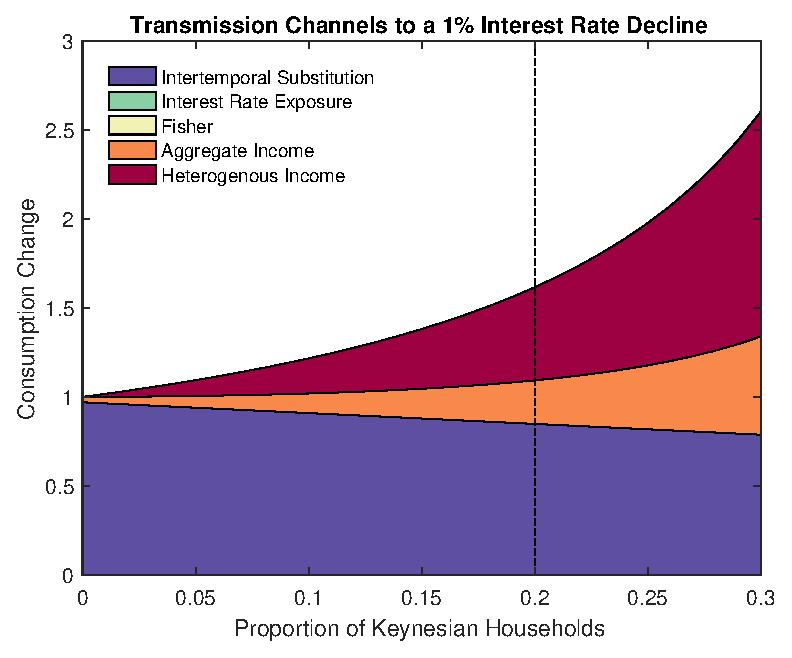
\includegraphics[scale=0.7]{../Matlab/DynareCode/Figures/ProportionKeynesian_sigma1.eps}
		\caption{Changing the Proportion of Keynesian Households, $\sigma=1$}
		\label{fig:ProportionKeynesian}
	\end{centering}
\end{figure}

This feature of the standard New Keynesian model, that markups are low during a boom and high during a recession, is not backed by empirical evidence and has led some away from price frictions and toward nominal wage frictions.\footnote{This point is emphasized in \cite{broer_2018} and motivates modeling choices in \cite{auclert_inequality_2018}}. While we are sympathetic to this approach, for this paper we maintain the sticky price assumption to stay close to the existing HANK literature. One way to remove this heterogeneous income channel completely would be to divide the income from capital and profits proportionally between the Keynesian and Ricardian households. In that model, the total consumption change would remain unchanged as the number of Keynesian households increased, with the intertemporal substitution channel decreases proportional to the share of Ricardian's in the economy and the aggregate income channel making up the remainder. While the channels would be different, in this model the aggregate dynamics would be \textit{identical} to the RANK model.

\subsection{Introducing Debt}
In this section we analyze what happens when the Keynesian households are allowed to take on debt equal to some fraction of their steady state income. For the remainder of this section we will fix the proportion of Keynesian households at 0.2, giving an economy-wide MPC of just over 20 percent. This number is chosen both because it is close to a number of the current theoretical HANK models, and a larger number causes indeterminacy problems for some parameterizations.\footnote{See \cite{gali_2004} for a detailed discussion on determinacy of TANK models.} However, we accept 0.2 is on the low end of empirical estimates.\footnote{A large literature aims to estimate MPCS. See \cite{johnson_household_2006}, \cite{parker_consumer_2013}, \cite{fagereng_mpc_2016} and \cite{ckConsumption} for a small selection of examples.} In figure \ref{fig:ProportionKeynesian} from the previous section, there is a dotted line drawn where the proportion of Keynesian households equals 0.2. This shows the size of the transmission channels for this section when there is no debt.

Figure \ref{fig:KeynesianDebt} shows how the size of the transmission channels change with the level of debt held by the Keynesian households, with the three panels showing this for decreasing elasticity of substitution.\footnote{The elasticity of substitution is equal to $1/\sigma$, so the three panels in figure \ref{fig:KeynesianDebt} represent an elasticity of substitution of 1, 0.5 and 0.33 respectively.} Starting with the left hand panel, we consider how the model behaves with an elasticity of substitution equal to one. The intercepts with the y-axis exactly correspond with the intercepts with the dotted line from figure \ref{fig:ProportionKeynesian}. This is the size of the transmission channels when a proportion 0.2 of households are Keynesian and these households have no debt. As in the previous section, the intertemporal substitution channel is slightly below one, while the income channels also play a significant role due to presence of Keynesian households. However, with no debt at the intersection with the y-axis both the interest rate exposure and Fisher channels are zero.

\begin{figure} 
	\begin{centering}
		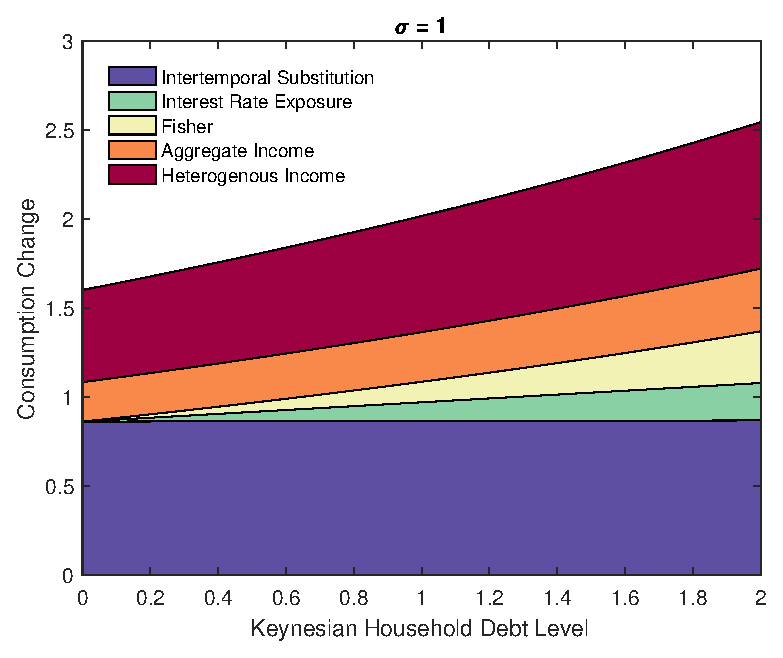
\includegraphics[scale=0.4]{../Matlab/DynareCode/Figures/KeynesianDebt_sigma1.eps}
		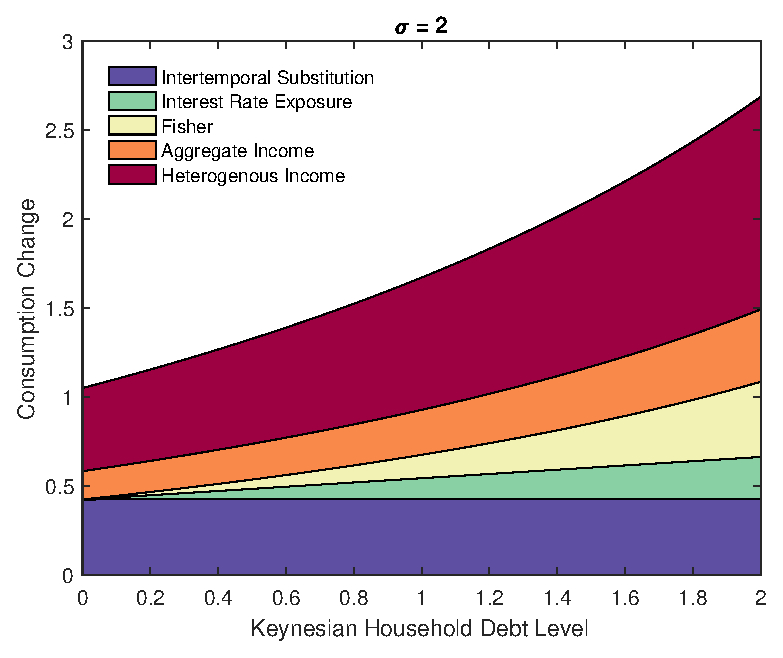
\includegraphics[scale=0.4]{../Matlab/DynareCode/Figures/KeynesianDebt_sigma2.eps}
		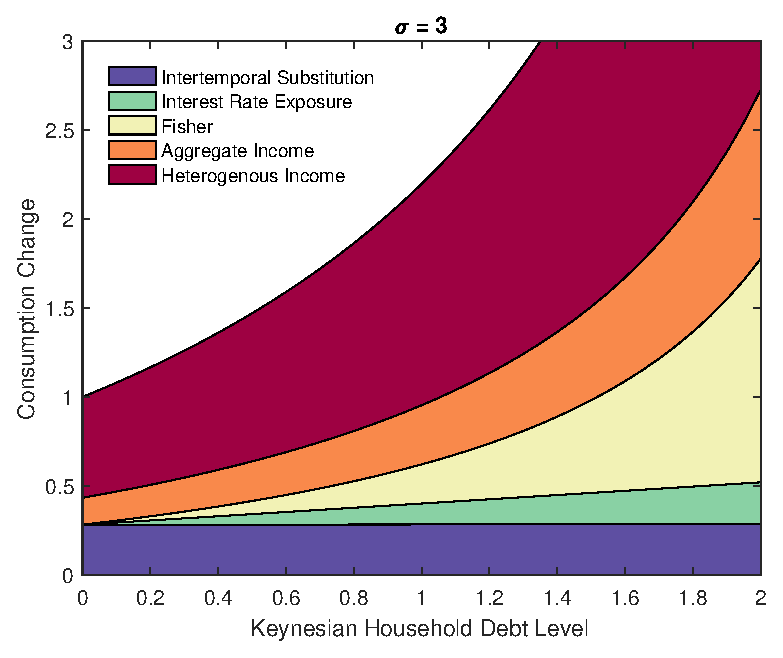
\includegraphics[scale=0.4]{../Matlab/DynareCode/Figures/KeynesianDebt_sigma3.eps}
		\caption{Changing the Debt of Keynesian Households}
		\label{fig:KeynesianDebt}
	\end{centering}
\end{figure}

As the quantity of debt that the Keynesian households can take on increases, both the interest rate exposure and Fisher channel start to become quantitatively important. Still looking at the left hand panel of figure \ref{fig:KeynesianDebt}, we see both of these channels growing, but they are still dominated by the intertemporal substitution channel. The two income channels grow in exact proportion to the other three channels, acting as a constant multiplier of the other three channels, no matter the quantity of debt. It may be useful to think of the transmission of monetary policy acting in stages. First aggregate demand is directly affected by the intertemporal substitution and interest rate exposure channels. The size of these channels depends only on the change in the interest rate, and is not changed as output and inflation change. The size of the Fisher channel is proportional to the amount of nominal debt, multiplied by the size of the overall change in income.\footnote{This is because inflation is proportional to the output gap in this model.} Finally the income channels are each a constant proportion of the total income change. We can think of intertemporal substitution and interest rate exposure as providing the initial `kick', which is then augmented by the Fisher and income channels.

The center and right panels of figure \ref{fig:KeynesianDebt} show the same channels, but when the elasticity of substitution is 0.5 and 0.33 respectively. The size of the intertemporal substitution channel is reduced in the same proportion, by 0.5 and 0.33 as the Ricardian households are now less happy to shift consumption between periods. However, the interest rate exposure channel remains exactly the same size as before. It is determined by the change in the borrowing cost along with the size of the debt, both of which are unchanged. The aggregate income channel is also exactly the same multiple of the other channels in all three panels, as is the Fisher channel.\footnote{The aggregate income multiplier is constant across both debt levels and intertemporal elasticity. The Fisher multiplier varies by debt level, but for any particular debt level it does not vary with intertemporal elasticity} The heterogeneous income multiplier grows significantly with $\sigma$. This is because the markup, and hence firm profits, become \textit{more} countercyclical with higher $\sigma$. Again, this feature of the standard New Keynesian model is undesirable and leads us here to be unable analyze the model under low elasticities of substitution that we believe to be more empirically reasonable.\footnote{See \cite{havranek_measuring_2015} for a meta-study for EIS estimates.}

This brings us to a broader point: the calibration of the elasticity of intertemporal substitution (EIS) in the standard New Keynsian model has been chosen to match aggregate data, despite the little micro evidence we have suggesting a much lower level. Figure \ref{fig:KeynesianDebt} shows why, in the absence of debt, a large EIS is required: with no debt the intertemporal substitution channel is the only `kick' to aggregate demand, so if this is small we need very large multipliers to get a sizable consumption response to monetary policy. If we make the EIS small, we need something else to take its place. Interest rate exposure is another `kick', that empirical evidence has shown could be large,\footnote{See \cite{auclert_monetary_2017} and \cite{ckConsumption}.}. By introducing interest rate exposure, we allow our models to use more micro-founded estimates of the EIS while still generating the kinds of aggregate responses estimated in the macro data.

\section{Relaxing the Fixed Capital Assumption}
Instead of a fixed amount of capital, K, allow for investment. If there are no costs to investment, then households will invest until the new capital stock gives risk to the changed interest rate, which will result in a very persistent change in the interest rate. We will need convex investment adjustment costs to avoid this persistence, and hope to show that reasonable calibrations result in little change in the capital stock and hence low interest rate persistence. Auclert did something like this in a previous version of his paper.

\subsection{The Model}
The model is identical to the baseline model, except for the fact that the Ricardian households are now able to invest in capital as well as nominal bonds. Aggregate investment at time $t$, $\text{Inv}_t$, along with the level of capital at time $t$, $K_t$, together determine the capital level at time $t+1$:
\begin{align}
\text{Inv}_t = \Phi\left(\frac{K_{t+1}}{K_t}\right) K_t
\end{align}
where $\Phi(1) =\delta$ is the per period depreciation, $\Phi'(1) =1$ and $\Phi''(1) =\psi_K >0 $ represents convex capital adjustment costs. It is the fact that capital in period $t+1$ is \textit{predetermined} in period $t$ that differentiates this model from the baseline model in terms of breaking the assumptions required for Auclert's sufficient statistics to hold. In steady state the investment share of income is $\overline{\textit{inv}} = \frac{\varepsilon-1}{\varepsilon} \frac{\delta \alpha}{1/\beta - (1-\delta)}$.\footnote{This comes from equating the steady-state return from investment with $1/\beta$, the steady-state real interest rate, and using the fact that in equilibrium the total income allocated to capital is equal to $\frac{\alpha}{1-\alpha}$ times the total income allocated to labor. For other steady-state ratios, equation \ref{c_K_n_K} remains the same, but \ref{c_K_ss} becomes $(\overline{c}_{K})^\sigma  \left(\frac{\overline{c}_{K}}{\xi^K}\right)^\psi = \left(\frac{\lambda}{1-\lambda}\right)^{\sigma+\psi}(1-\overline{\textit{inv}}-\overline{c}_{K})^\sigma  (1-\frac{\overline{c}_{K}}{\xi^K})^\psi$ and $\overline{c}_{R}=1-\overline{\textit{inv}}-\overline{c}_{K}$, taking account of the fact that investment now takes a chunk out of output which is no longer equal to aggregate consumption.}

\subsection{Changes Relative to the Linear Baseline Model}
Given nominal interest rate and inflation expectations, the individual optimization problems for both Ricardian and Keynesian households, as well as firms, remains identical to the baseline model. That results in equations \ref{euler_R_linear}, \ref{NKphillips_linear}, \ref{budget_constraint_K_linear}, \ref{foc_hours_R_linear} and \ref{foc_hours_K_linear} remaining unchanged. Differences occur in aggregation.

As the natural level of output (output that would occur with flexible prices) is no longer constant, the output gap, $\tilde{y}$, is no longer equal to output. The model needs equations to define the natural level output and the output gap:\footnote{Natural output is derived from the fact that under flexible prices, the markup over marginal cost will be constant ($\frac{\varepsilon}{\varepsilon-1}$).}
\begin{align}
y^{n} &= \frac{\alpha(1+\psi)}{\sigma(1-\alpha) + \psi + \alpha} k_{t} \label{y_nat_linear} \\
\tilde{y}_t &= y_t - y^{n}	\label{output_gap_linear}
\end{align}
Futhermore, the aggregate production function, equation \ref{production_linear}, now includes capital:
\begin{align}
\tilde{y}_t &= \alpha k_t +  (1-\alpha)n_t  \label{production_capital_linear}
\end{align}
Aggregation of output now includes the capital share, so equation \ref{agg_C_linear} is replaced by:
\begin{align}
y_t &= \overline{c}_{K} c^K_t + \overline{c}_{R} c^R_t + \overline{\textit{inv}} \ \textit{inv}_t \label{agg_Y_linear}
\end{align}
The law of motion for capital is introduced to the model:
\begin{align}
\delta \ \textit{inv}_t = k_{t+1} - (1-\delta) k_{t}    \label{lom_capital}
\end{align}
As is the equation for the shadow price of capital, $q_t$, determined by the convexity of adjustment costs:
\begin{align}
q_t = \psi_K (k_{t+1}-k_t)	\label{shadow_K}
\end{align}
Finally we require an equation to equate the expected return on investment with the expected real return on nominal bonds:
\begin{align}
r_t + q_t = \beta (1-\delta) \mathbb{E}_t q_{t+1} + (1 - \beta (1-\delta)) (\mathbb{E}_t (w_{t+1} + n_{t+1}) - k_{t+1})	\label{return_K}
\end{align}





\section{Assumptions on Government Expenditure}
The sufficient statistics rely heavily on the tax rebate assumption that an extra government revenues are immediately paid back in equal lump sums to all households. We need to relax this, and hope to show in the TANK model that a version of the sufficient statistics where we do not assume any rebate, holds fairly well (as long as the number of constrained households is quite high).

\section{Nature of the Borrowing Constraint}
Here I want to show the effect of changing the borrowing constraint from a proportion of next periods income to a proportion of today's income. I think this will have the effect of delaying the constrained households response by one period, but perhaps the average response over two periods may be similar?

\section{A Simple HANK Model}
Here is where we put the results from our HANK model. For the moment we should perhaps stick to the one asset version. One key thing to show is again that there is little persistence in the dynamics following a transitory shock. In the IRFs we see a slight hump in period 2 which we should try and understand (I think it is due to a change in the distribution of wealth).

\subsection{Households}

\section{Unhedged Interest Exposure in Existing HANK Models}
By now we have hopefully convinced the reader that the sufficient statistics do a reasonable job in a variety of models as long as there is no `artificial' persistence in the interest rate shock.

We now want to show that the joint distribution of unhedged interest rate exposure and MPCs is very poorly calibrated in our current generation of HANK models. Furthermore, the evidence suggests this joint distribution is very persistent over time, in contrast to many two asset models which suggest households come in and out of their liquidity constrained position regularly.


\section{Conclusion}
Lots of future research to do!


\processdelayedfloats

\small
\bibliography{AllPapers}
\normalsize

\end{document}









